\chapter{На каких языках программирования пишутся операционные системы}
\label{ch:operating-sysmets}

В статье исследуется объект Викиданных <<операционная система>> (operating system) и его свойства. В каждом из разделов представлены задачи, решённые с помощью SPARQL-запросов. В их числе: нахождение экземпляров объекта <<операционная система>>, построение списка операционных систем (ОС) по предку, по времени создания, по языку, на котором написана ОС. Также построена гистограмма, показывающая количество программ, написанных на том или ином языке программирования, и долю того, сколько из них работает под той или иной ОС. У многого программного обеспечения не указан язык программирования, на котором оно разрабатывалось. Для улучшения результатов решения вышеописанных задач отдельные объекты Викиданных были дополнены свойством <<язык программирования>>.

\section{Полнота данных}
По данным на 2017 год с сайта www.operating-system.org удалось установить что существует порядка 611 операционных систем (не учитывая дистрибутивы Linux'а, коих количество превышает количество самих операционных систем). В то время как викиданные содержат информацию лишь о 510 операционных системах. И если просмотреть достаточно большое количество объектов из запрос, то станет ясно еще и то, что много из них еще и не очень хорошо заполнены, а то и вовсе практически пусты.

В 2020 году викиданные содержат информацию о 1086 операционных системах, что свидетельствует о значительных изменениях, однако большое количество объектов по-прежнему плохо заполнены. Из этого можно сделать вывод о неполноте викиданных.

\section{Языки программирования, используемые для написания операционных система}
Если взглянуть на количество операционных систем, для которых указано свойство <<язык программирования>>, то можно увидеть что из 1086 объектов это свойство заполнено лишь у 116. Но по существующим данным на рис.~\ref{fig:count-os-written-on-languages} можно определить, что большинство операционных систем написаны на языке программирования C. 
\begin{figure*}[h!]
	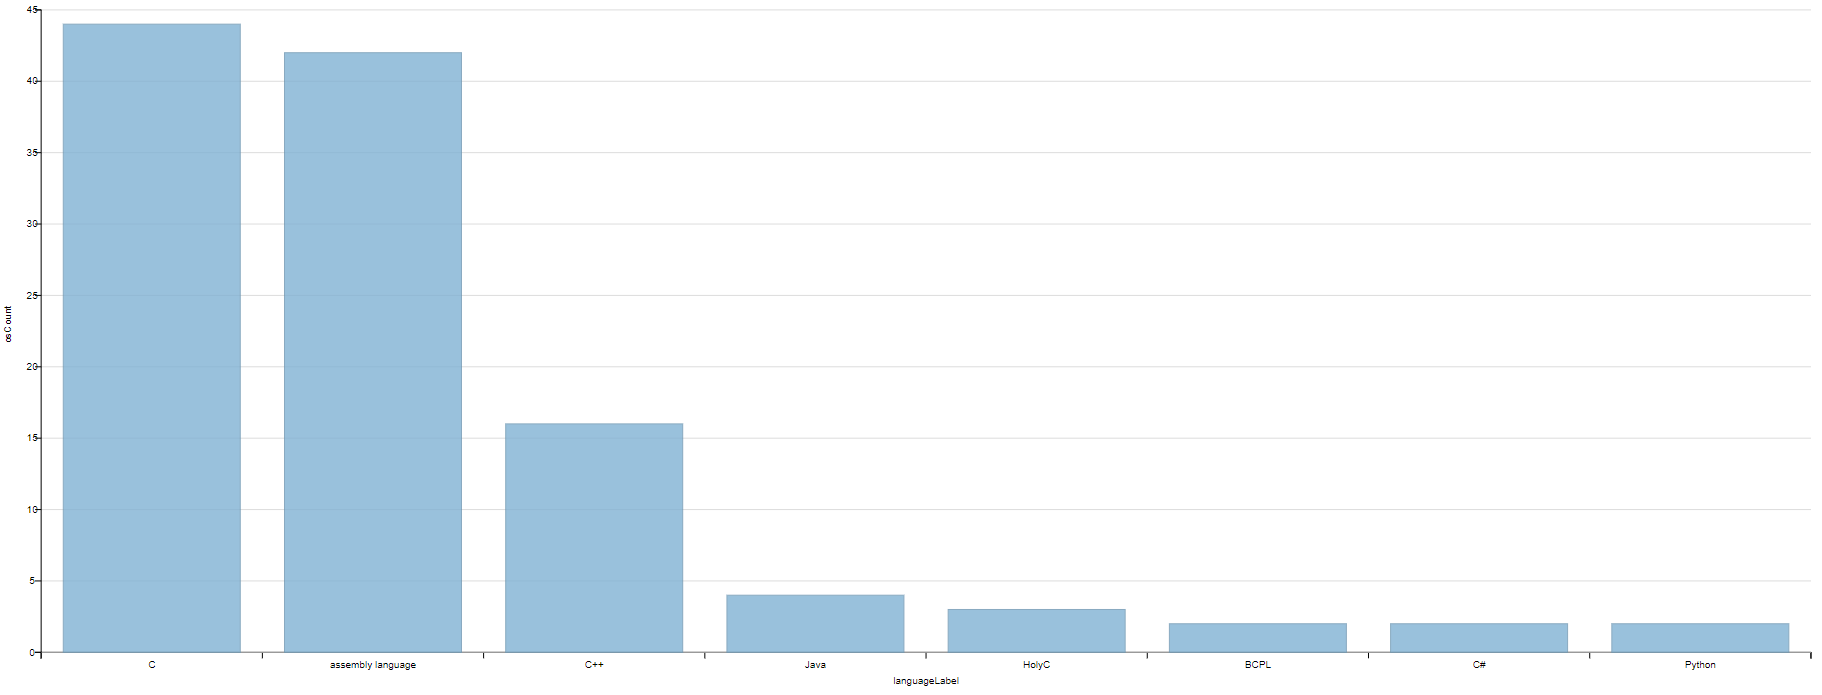
\includegraphics{./chapter/operating_system/count-os-written-on-languages.png}
	\caption{Количество операционных систем, написанных на языках программирования (данные на 2020 год.)}
	\label{fig:count-os-written-on-languages}
\end{figure*}


Гистограмма на рисунке~\ref{fig:count-software-written-on-languages} позволяет увидеть для каждого языка программирования количество программ, которые были на нем написаны, а также под какими ОС работают данные программы. Из графика видно, что наибольшее число программ пишется на языках: С++ (2503 программ), Си (2566 программ), Java (799 программ), Python (717 программ),  JavaScript (344 программы).

Рассмотрим каждый из этих языков подробнее.

Большая часть программ на языке С++ пишется под windows (472 программы) и macOs (300 программ). Несмотря на то, что язык был разработан в 1972, он пока не теряет своей популярности за счет, вероятно, того, что используется для написания низкоуровневых приложений, т.к. по "близости" к аппаратному уровню уступает разве что ассемлеру.

Большая часть программ на языке С++ пишется под macOS (400 программ) и windows (700 программ) и Linux (400 программы). Вероятно, С++ будет лидировать еще долгое время, т.к. на текущий момент он используется для решений, требующих высокой производительности, чего не позволяют высокоуровневые языки, как Java или C\#.

Большая часть программ на языке Java пишется под macOS (196 программ) и Андроид (156 программ). Вероятно, Java пользуется популярностью за счет переносимости кода, т.е. код на Java запустится на любой машине с установленной JVM.

Большая часть программ на языке JavaScript пишется под macOS (100 программ) и Андроид (60 программ) и iOS (40 программ). Как правило, используется для написания клиентской части веб-приложений, что разработке сложных веб-приложений приводит к снижению нагрузки на сервер и увеличению скорости работы приложения.

Большая часть программ на языке Python пишется под macOS (212 программ) и Linux (107 программ). Высокоуровневый язык с низким порогом вхождения. Используется, например, для написания веб-приложений и анализа данных.

Глядя на гистограмму, можно сделать вывод, что каждый из данных языков занял свою "нишу" в области разработки ПО и применяется для определенного круга задач. Также вижно, что большая часть ПО пишется под macOS (900 программ), windows (1500 программ), Linux (1200 программ) или Андроид (300 программ).


\begin{figure*}[h!]
	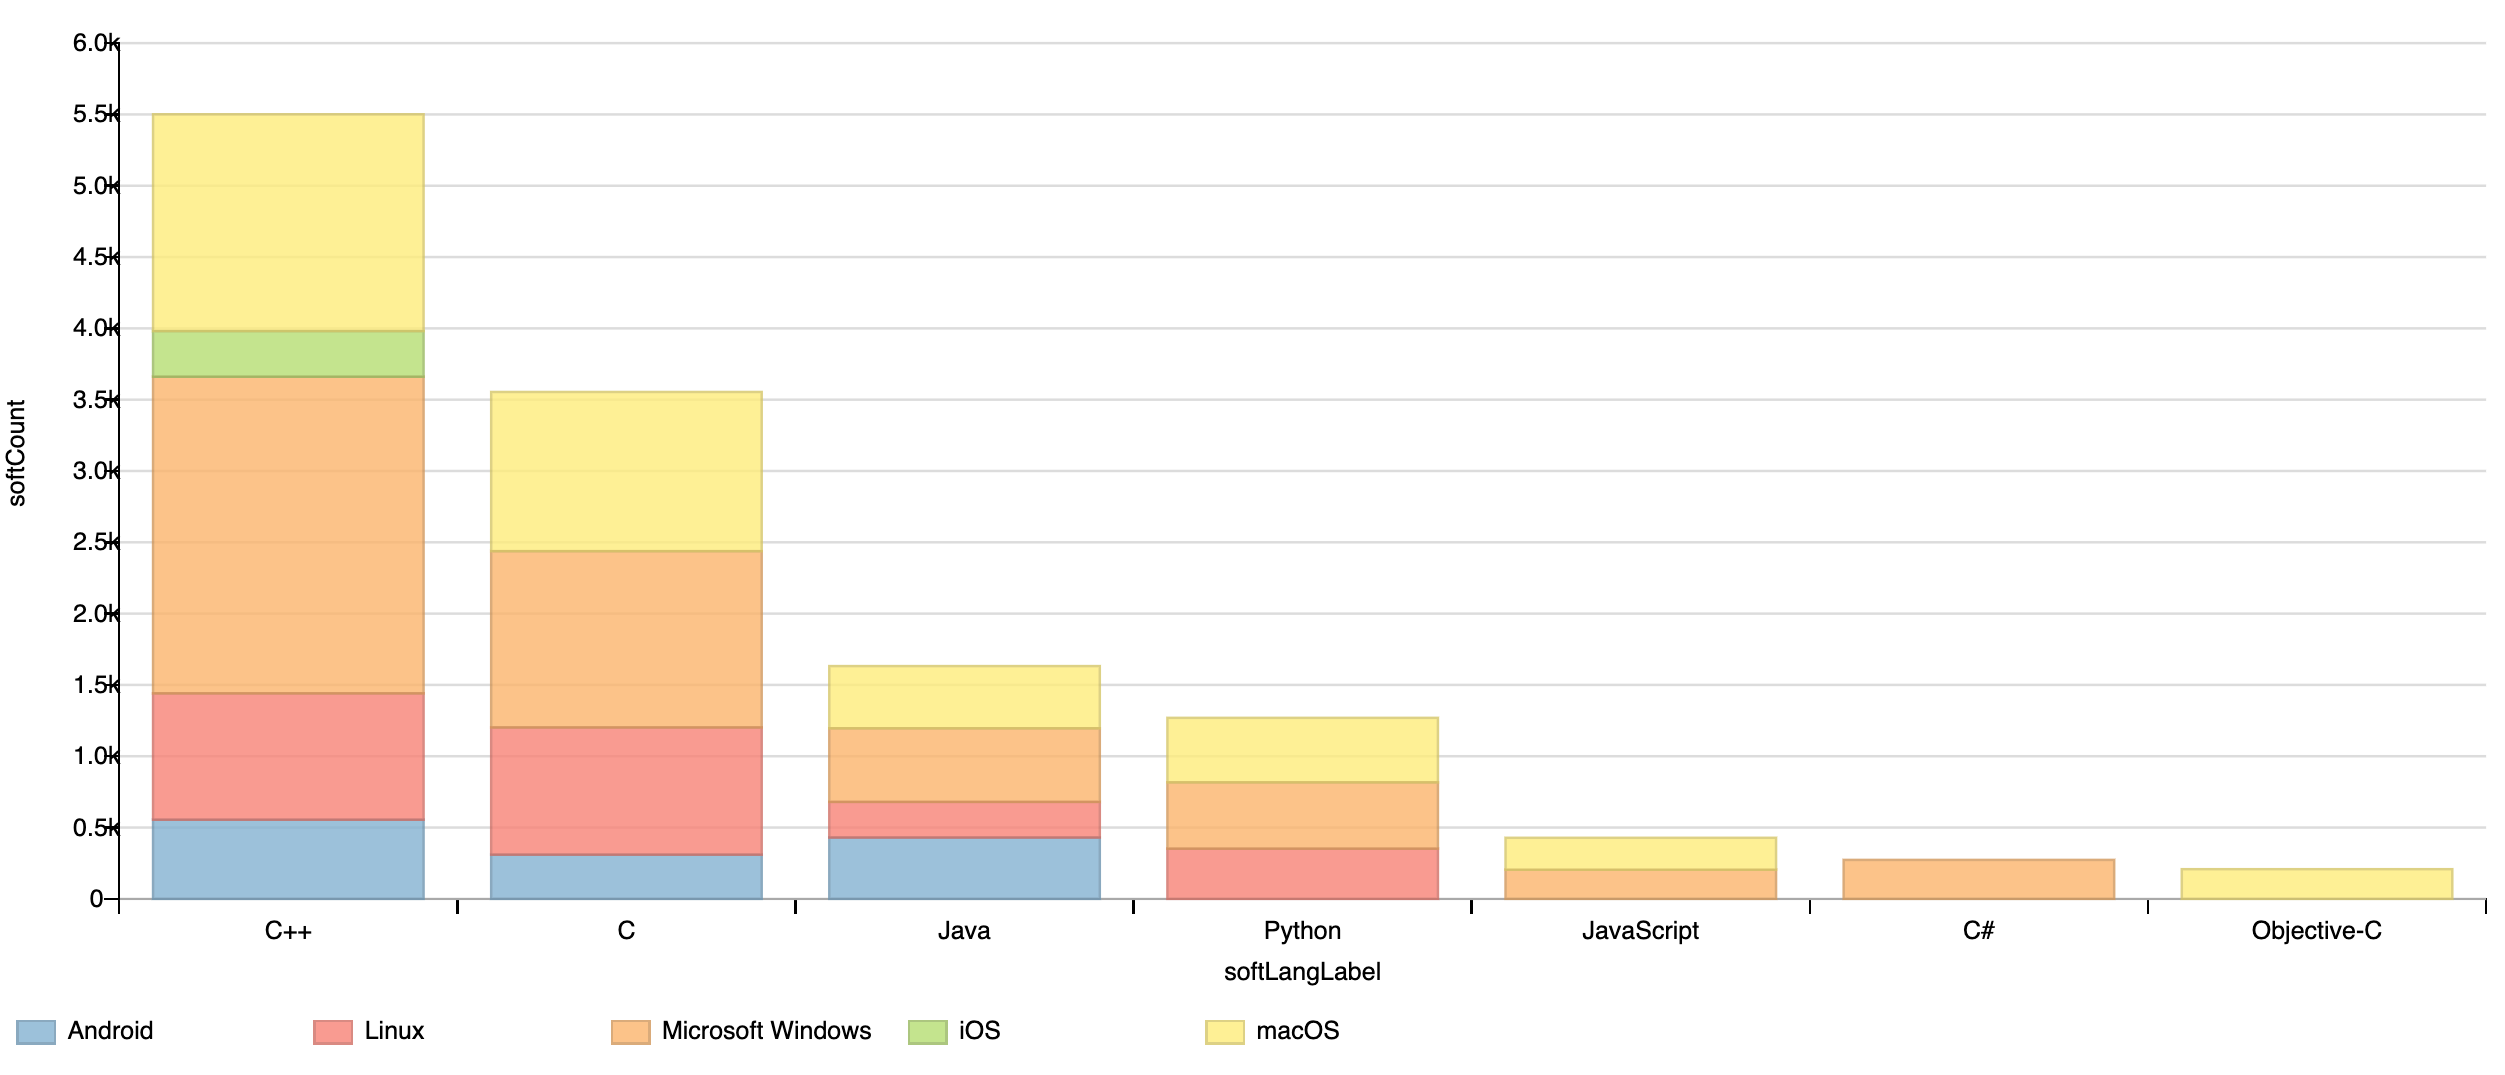
\includegraphics{./chapter/operating_system/Programming-languages-and-count-of-programms-written-on-them-and-OS-2020.png}
	\caption{Языки программирования и количества ОС, под которыми работают программы, написанные на них 2020 год.}
	\label{fig:count-software-written-on-languages}
\end{figure*}
